Classic magnetism question.

\begin{parts}
	\part Superexchange: in some materials where the magnetic species have no direct orbital overlaps, an intermediate non-magnetic species (e.g. \ion{O}{$2-$}) will facilitate an indirect exchange such that there is a kinematic advantage in an antiferromagnetic order.
	\begin{figure}[H]
		\centering
		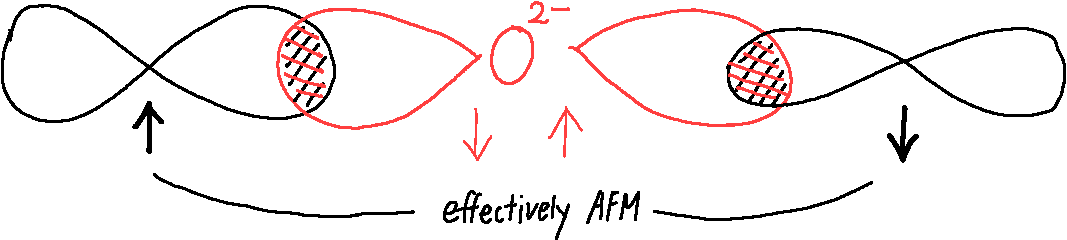
\includegraphics[width=.7\linewidth]{q1-superexchange}
	\end{figure}
	
	Heisenberg exchange: $\mathcal{H} = \sum_{i,j} J/2 \, \mathbf{S}_i \cdot \mathbf{S}_j$ where $1/2$ is due to overcounting.
	
	In mean field theory we may treat the spins as classical vectors, so:
	\begin{align}
		\mathcal{H}_{J_2} &= 4 \cdot \frac{J_2}{2} S^2 \cos\theta \label{eqn:q1-heisenberg-j2} \notag \\
		&= 2 J_2 S^2 \cos\theta \\[1em]
		\mathcal{H}_{J_1} &= 2 \cdot \frac{J_1}{2} S^2 \cos 2\theta \label{eqn:q1-heisenberg-j1} \\
		&= J_1 S^2 \underbracket{\sbracket{2\cos^2 \theta - 1}}_{f(\theta)} \notag
	\end{align}
	
	So energy per spin in spiral order:
	\begin{gather}
		E_\textnormal{spiral}(\theta) = 2J_2 S^2 \cos\theta + J_1 S^2 \sbracket{2\cos^2 \theta - 1} \notag \\
		\pderi{E_\textnormal{spiral}}{\theta} = -2J_2 S^2 \sin\theta - 4J_1 S^2 \cos\theta \sin\theta = 0 \mtext{at equilibrium} \notag \\
		\Rightarrow -2S^2 \sin\theta \sbracket{J_2 + 2J_1 \cos\theta} = 0 \notag \\
		\Rightarrow \sin\theta = 0 \mtext{(AFM state)} \qquad \textnormal{or} \qquad \cos\theta = -\frac{J_2}{2J_1} \label{eqn:q1-theta-equilibrium}
	\end{gather}
	
	Note that the spiral solution vanishes when $\abs{\cos\theta} > 1$:
	\begin{gather*}
		-\frac{J_2}{2J_1} < -1 \\
		\Rightarrow \frac{J_1}{J_2} < \frac{1}{2}
	\end{gather*}
	Thus the spiral state would be more stable than the AFM state for $J_1 / J_2 > 1/2$.
	
	Also for large $J_1 / J_2$:
	\begin{equation*}
		\lim_{J_1 \to \infty} \cos\theta = \lim_{J_1 \to \infty} -\frac{J_2}{2J_1} = 0
	\end{equation*}
	Thus we have a limiting value of
	\begin{equation*}
		\lim_{J_1/J_2 \to \infty} \theta = \frac{\pi}{2}
	\end{equation*}
	
	Sketch of $\theta$ against $J_1 / J_2$:
	\begin{figure}[H]
		\centering
		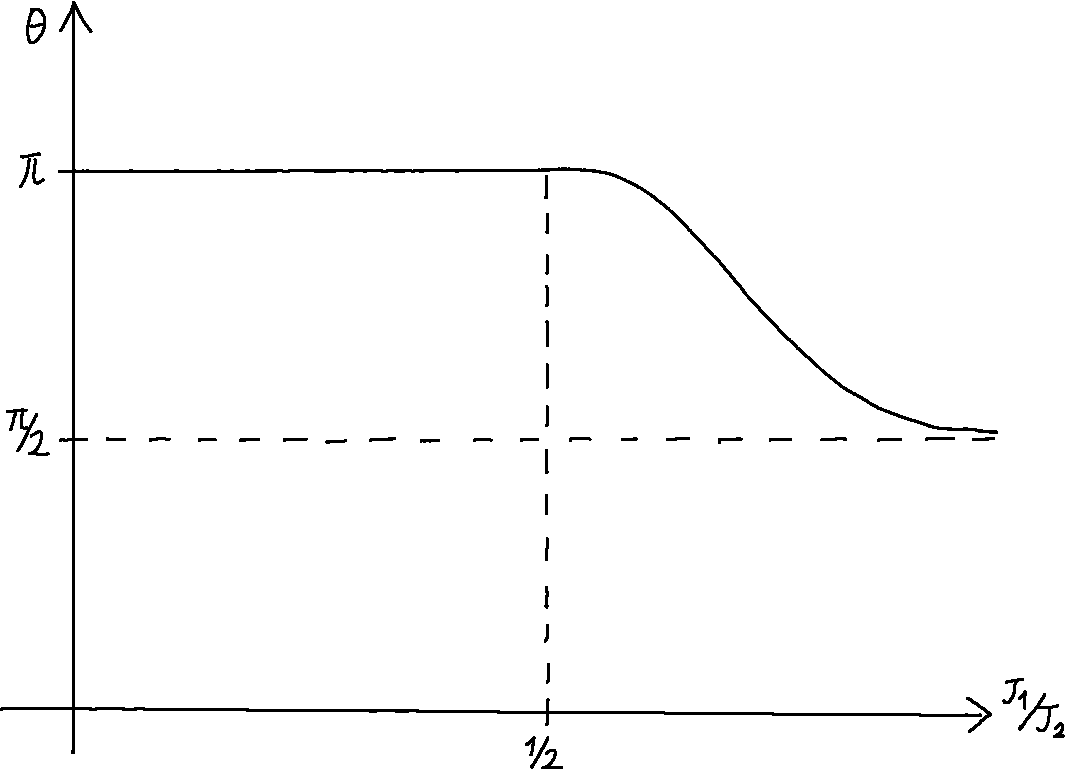
\includegraphics[width=.8\linewidth]{q1-afm}
	\end{figure}
	
	\part Similarly, by realising that Figure II depicts just the component $S \sin\alpha$, we may rewrite the interaction terms \eqref{eqn:q1-heisenberg-j2} and \eqref{eqn:q1-heisenberg-j1}:
	\begin{align*}
		\mathcal{H}_{J_1} &= 2 \cdot \frac{J_1}{2} S^2 \sbracket{\cos 2\theta \sin^2 \alpha + \cos^2 \alpha} \\[1em]
		\mathcal{H}_{J_2} &= 4 \cdot \frac{J_2}{2} S^2 \sbracket{\cos \theta \sin^2 \alpha + \cos^2 \alpha}
	\end{align*}
	
	So the energy terms become:
	\begin{gather*}
		E = E_\textnormal{spiral} \sin^2 \alpha + \rbracket{J_1 + 2J_2} S^2 \cos^2 \alpha + \underbracket{\rbracket{-g \bohrmagneton \mathbf{S}} \cdot \mathbf{B}}_{-g \bohrmagneton BS \cos\alpha} \\
		\pderi{E}{\alpha} = 2 E_\textnormal{spiral} \sin\alpha \cos\alpha - \rbracket{J_1 + 2J_2} 2S^2 \sin\alpha \cos\alpha + g \bohrmagneton BS \sin\alpha = 0 \mtext{at equilibrium} \\
		\Rightarrow \sin\alpha = 0 \mtext{(paramagnetic regime)} \qquad \textnormal{or} \qquad \cos\alpha = \frac{g \bohrmagneton BS}{2\rbracket{J_1 + 2J_2}S^2 - 2E_\textnormal{spiral}} \\
		\cos\alpha = \frac{g \bohrmagneton B}{2\rbracket{J_1 + 2J_2} S - 4J_2 S \cos\theta_\textnormal{eq} - 2J_1 S \rbracket{2 \cos^2 \theta_\textnormal{eq} - 1}} \\
		= \frac{g \bohrmagneton B}{\sbracket{2\rbracket{J_1 + 2J_2} + \frac{J_2^2}{J_1} + 2J_1} S}
	\end{gather*}
	where $\theta_\textnormal{eq}$ is the value of $\theta$ at equilibrium from \eqref{eqn:q1-theta-equilibrium}.
	
	Saturation occurs when $\cos\alpha = 1 \Rightarrow \alpha = 0$:
	\begin{align*}
		\Rightarrow B_\textnormal{sat} &= \frac{2S}{g \bohrmagneton} \sbracket{J_1 + 2J_2 + \frac{J_2^2}{2J_1} + J_1} \\
		&= \frac{2S}{g \bohrmagneton} \sbracket{2J_1 + 2J_2 + \frac{J_2^2}{2J_1}}
	\end{align*}
	
	Sketch of $M \cos\alpha$ against $B$:
	\begin{figure}[H]
		\centering
		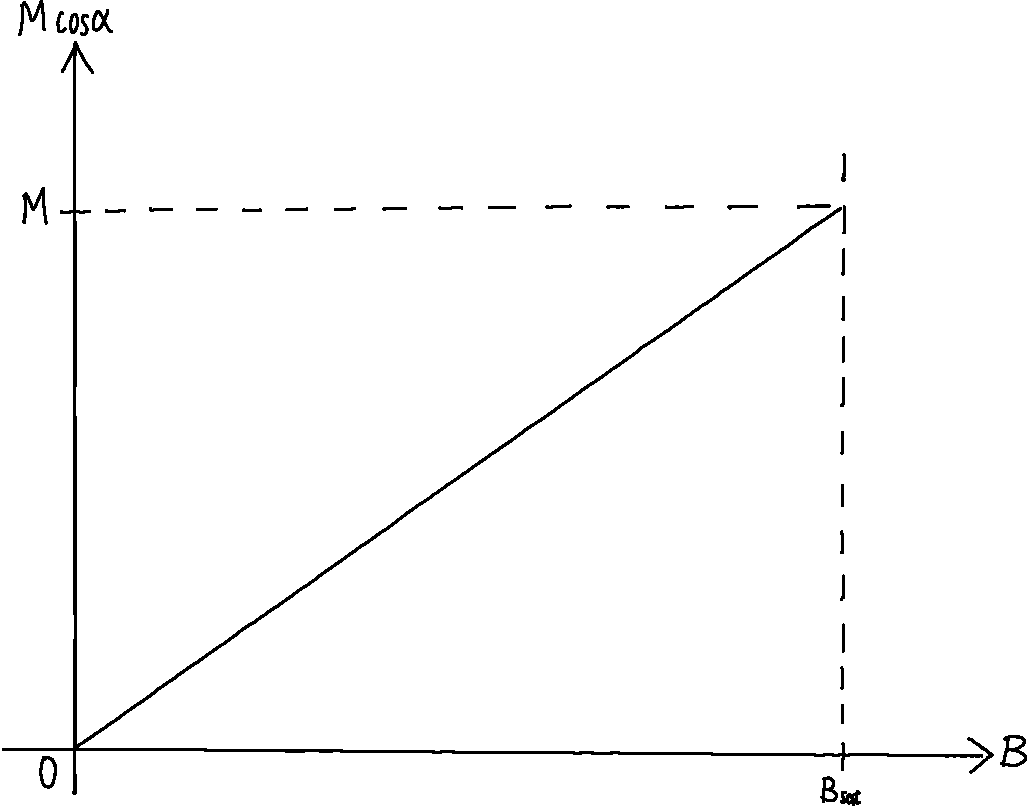
\includegraphics[width=.7\linewidth]{q1-magnetisation}
	\end{figure}
	
	\part \todo To determine the alignment of the spins, one may perform a polarised neutron scattering and measure the relative intensities of scattering.
\end{parts}